This assignment is about 2-dimensional vectors. A 2-dimensional vector
(henceforth just called a vector) is a geometrical object consisting
of a length and a direction. Typically, a vector is represented as
a pair of numbers, $\vec v  = (x, y)$, where its length and direction
are found as,
\begin{align}
  \text{len}(\vec v) &= \sqrt{x^2+y^2}
  \\\text{ang}(\vec v) &=\text{atan2}(y, x)
\end{align}
Vectors are often drawn as arrows with a head and a tail. In the
Cartesian coordinate system, if the tail is placed at $(0, 0)$, then
the head will be at $(x, y)$. Addition of vectors is performed
elementwise:
\begin{align}
  \vec v_1 &= (x_1, y_1)
  \\\vec v_2 &= (x_2, y_2)
  %\\a \vec v_1 &= (a x_1, a y_1)
  \\\vec v_1 + \vec v_2 &= (x_1+x_2, y_1+y_2)
  %\\\vec v_1 \cdot \vec v_2 &= x_1 x_2 +  y_1y_2
\end{align}
Addition can also be drawn, as shown in \Cref{fig:vectorAddition}.
\begin{figure}[h]
  \centering
  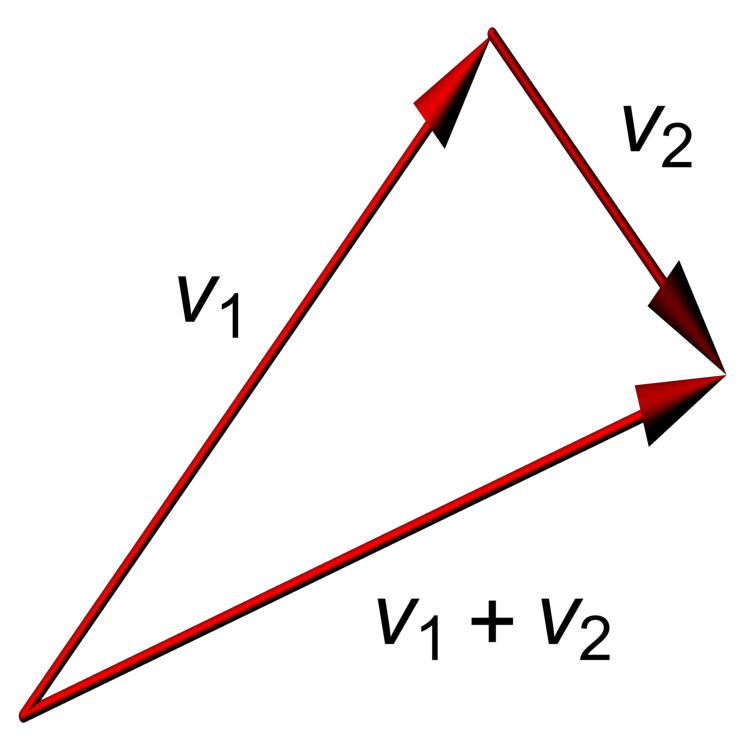
\includegraphics[width=0.33\textwidth]{vectorAddition}
  \caption{An illustation of vector addition.}
  \label{fig:vectorAddition}
\end{figure}
